\documentclass[11pt]{article}

\usepackage[lmargin=0.75in, rmargin=1in, tmargin=1.25in, bmargin=1in]{geometry}
\usepackage[english]{babel}
\usepackage[utf8]{inputenc}

\usepackage{amsfonts}
\usepackage{amsmath}
\usepackage{bm}
\usepackage{booktabs}
\usepackage[labelsep=period]{caption}
\usepackage{enumitem}
\usepackage{fancyhdr}
\usepackage{graphicx}
\usepackage{lastpage}
\usepackage{listings}
\usepackage[svgnames]{xcolor}
\usepackage{float}
\usepackage{array}
\usepackage{subcaption}
\newcolumntype{P}[1]{>{\centering\arraybackslash}p{#1}}
\newcolumntype{M}[1]{>{\centering\arraybackslash}m{#1}}

% For formatting C++ code listings ---------------------------
\lstdefinestyle{customCpp}{
    language=C++,
    keywordstyle=\color{RoyalBlue},
    basicstyle=\footnotesize\ttfamily,
    commentstyle=\color{Green}\ttfamily,
    rulecolor=\color{black},
    numbers=left,
    numberstyle=\tiny\color{gray},
    stepnumber=1,
    numbersep=8pt,
    showstringspaces=false,
    breaklines=true,
    frame = tb,
    belowcaptionskip=5pt,
    belowskip=3em,
    gobble=10,
}

% For turning enumerated lists into Problem titles --------------
\renewcommand{\labelenumi}{\textbf{\arabic{enumi}.}}
\renewcommand{\labelenumii}{(\alph{enumii})}
\setlength\parindent{24pt}
\newcommand{\forceindent}{\leavevmode{\parindent=1em\indent}}

% Enumerated list indents:
% Problems:    [leftmargin=0.9in]
% Subproblems: [leftmargin=0.3in]


% Document Details ----------------------------------------------
\author{Eli Case}
\title{MECH 450 -- Homework 1}
\date{September, 5, 2023}
\makeatletter


% Setup headers -------------------------------------------------
\pagestyle{fancy}
\fancyhf{} % Clear the headers and footers
\lhead{\@author}
\chead{\@title}
\rhead{\@date}
\cfoot{Page \thepage\ of \pageref{LastPage}}
\setlength{\headheight}{15pt}
\setlength{\headsep}{20pt}

\fancypagestyle{plain}{
	\fancyhf{}
	\setlength{\headheight}{15pt}
	\setlength{\headsep}{0pt}
	\renewcommand{\headrulewidth}{0pt}
	\cfoot{\vspace{2mm}Page \thepage\ of \pageref{LastPage}}
}


\begin{document}
\flushleft
\thispagestyle{plain}

From: \@author

Date: \@date

Subject: \@title

\makeatother
\medskip
\hrule
\medskip

\begin{enumerate}[leftmargin=0.3in]

   \item % Problem 1
   \begin{enumerate}
    We are given a point robot in a workspace, $W$, with a set of obstacles $WO_i$, $i \in \{1, 2, ..., m\}$ that is within the radius of the $d(q_{start}, q_{goal})$, and the remaining obstacles, $WO_j$, $j \in \{m +1,..., n\}$ for a total of $n$ obstacles. We can conclude that the maximum number of obstacles the robot will encounter using the BUG 1 algorithm is $m$ obstacles. \break 

   To understand why the answer is $m$ obstacles, consider the following case shown below in Figure \ref{fig:1}. \break 

   \begin{figure}[H]
      \centering
      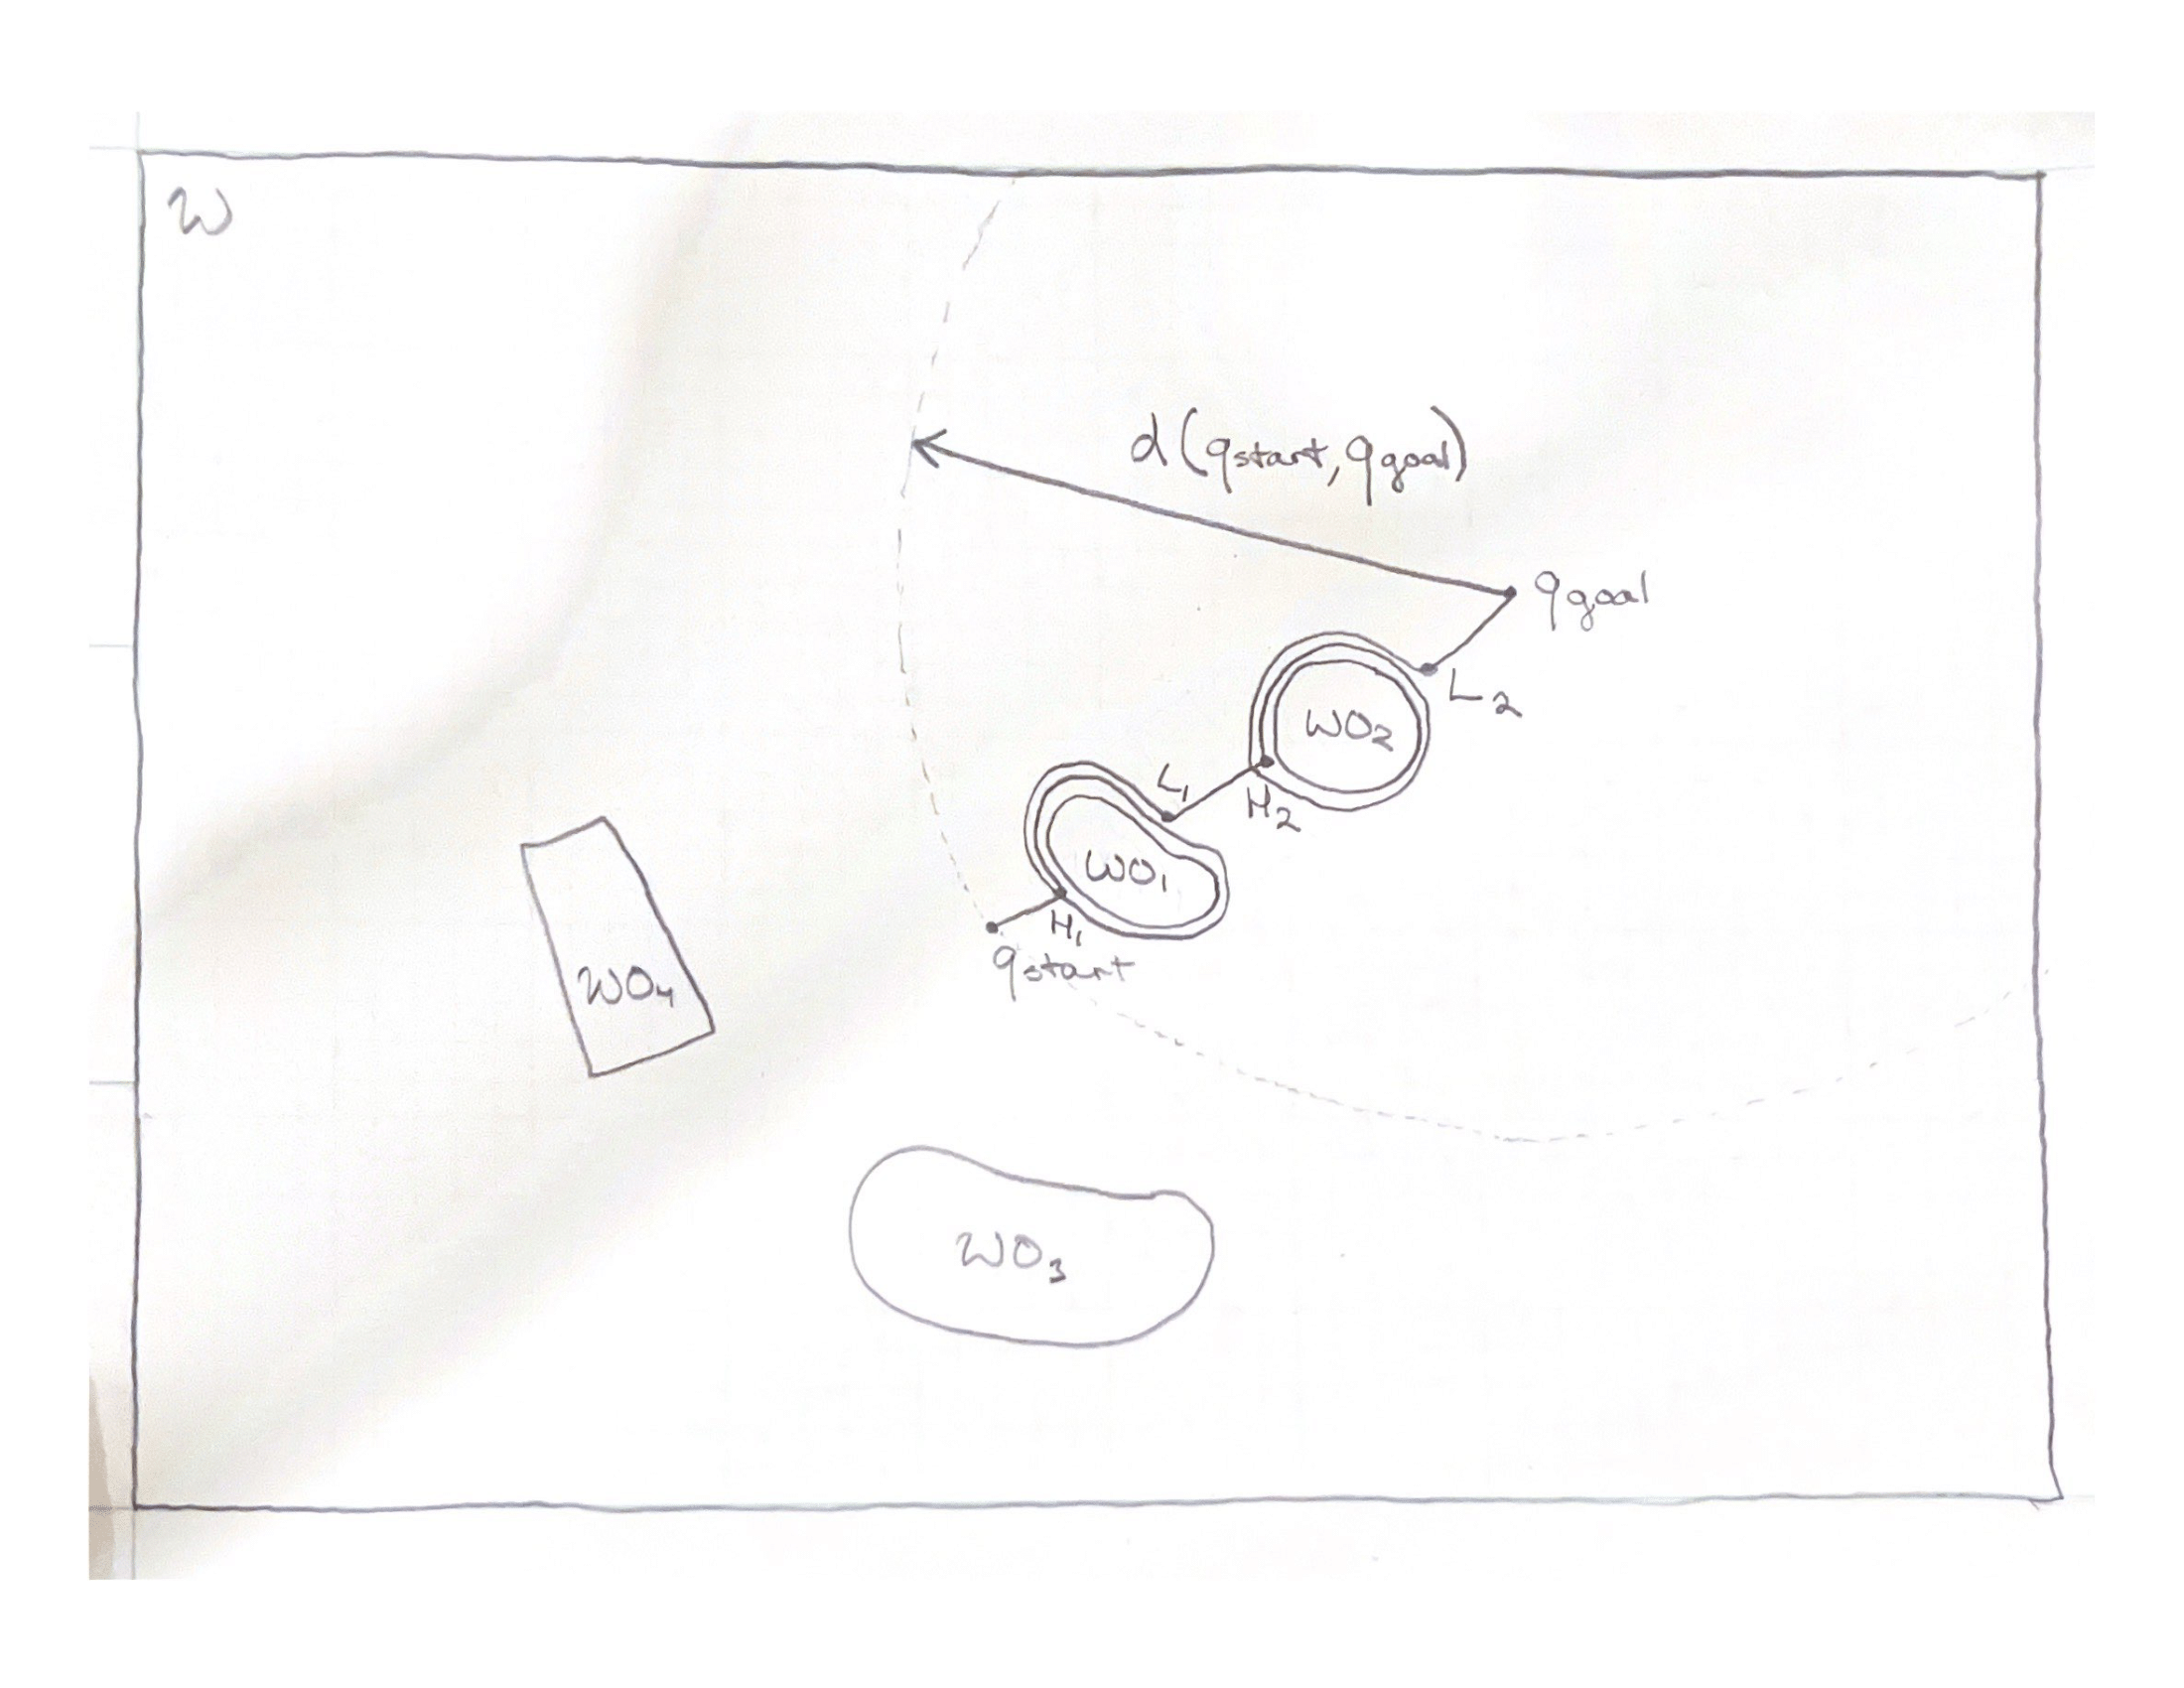
\includegraphics[width=11cm]{figures/problem1.png}
      \caption{Example Workspace}
      \label{fig:1}
   \end{figure}
    
   In this example, we consider a series of 4 obstacles, 2 of which are within the radius of $d(q_{start}, q_{goal})$, so then $m = 2$, $n = 4$. From this example we can see for the obstacles within the radius of $d(q_{start}, q_{goal})$, the BUG 1 algorithm generates a leave point, $q^{L_i}$, at a closer distance to the goal than the corresponding hit point $q^{H_i}$. Consequently, the BUG 1 algorithm does not interact with the obstacles outside the radius $d(q_{start}, q_{goal})$. \break

   For the general case of $n$ obstacles, we can make the following proposition from observing the last example. \break 

   \textit{Since BUG 1 generates a leave point, $q^{L_i}$, closer to the goal that the corresponding hit point, $q^{H_i}$, for the obstacle $WO_i$ with $i \in \{i,...,m\}$, the obstacles $WO_j$ with $j \in \{m+1,...,n\}$ are not encountered when using BUG 1.} \break

   The fact that $q^{L_i}$ is always closer to the goal than $q^{H_i}$ is by design of the BUG 1 algorithm. As a result, we conclude that the most obstacles encountered will be $m$ obstacles.

  \end{enumerate} % End of Problem 1 subpoints

  \item % Problem 2
  \begin{enumerate}
    Below in Figure \ref{fig:2}, the trajectories for produced by Bug 1, Bug 2, and Tangent Bug with infinite sensor range are shown.
   
   \begin{figure}[H]
      \centering
      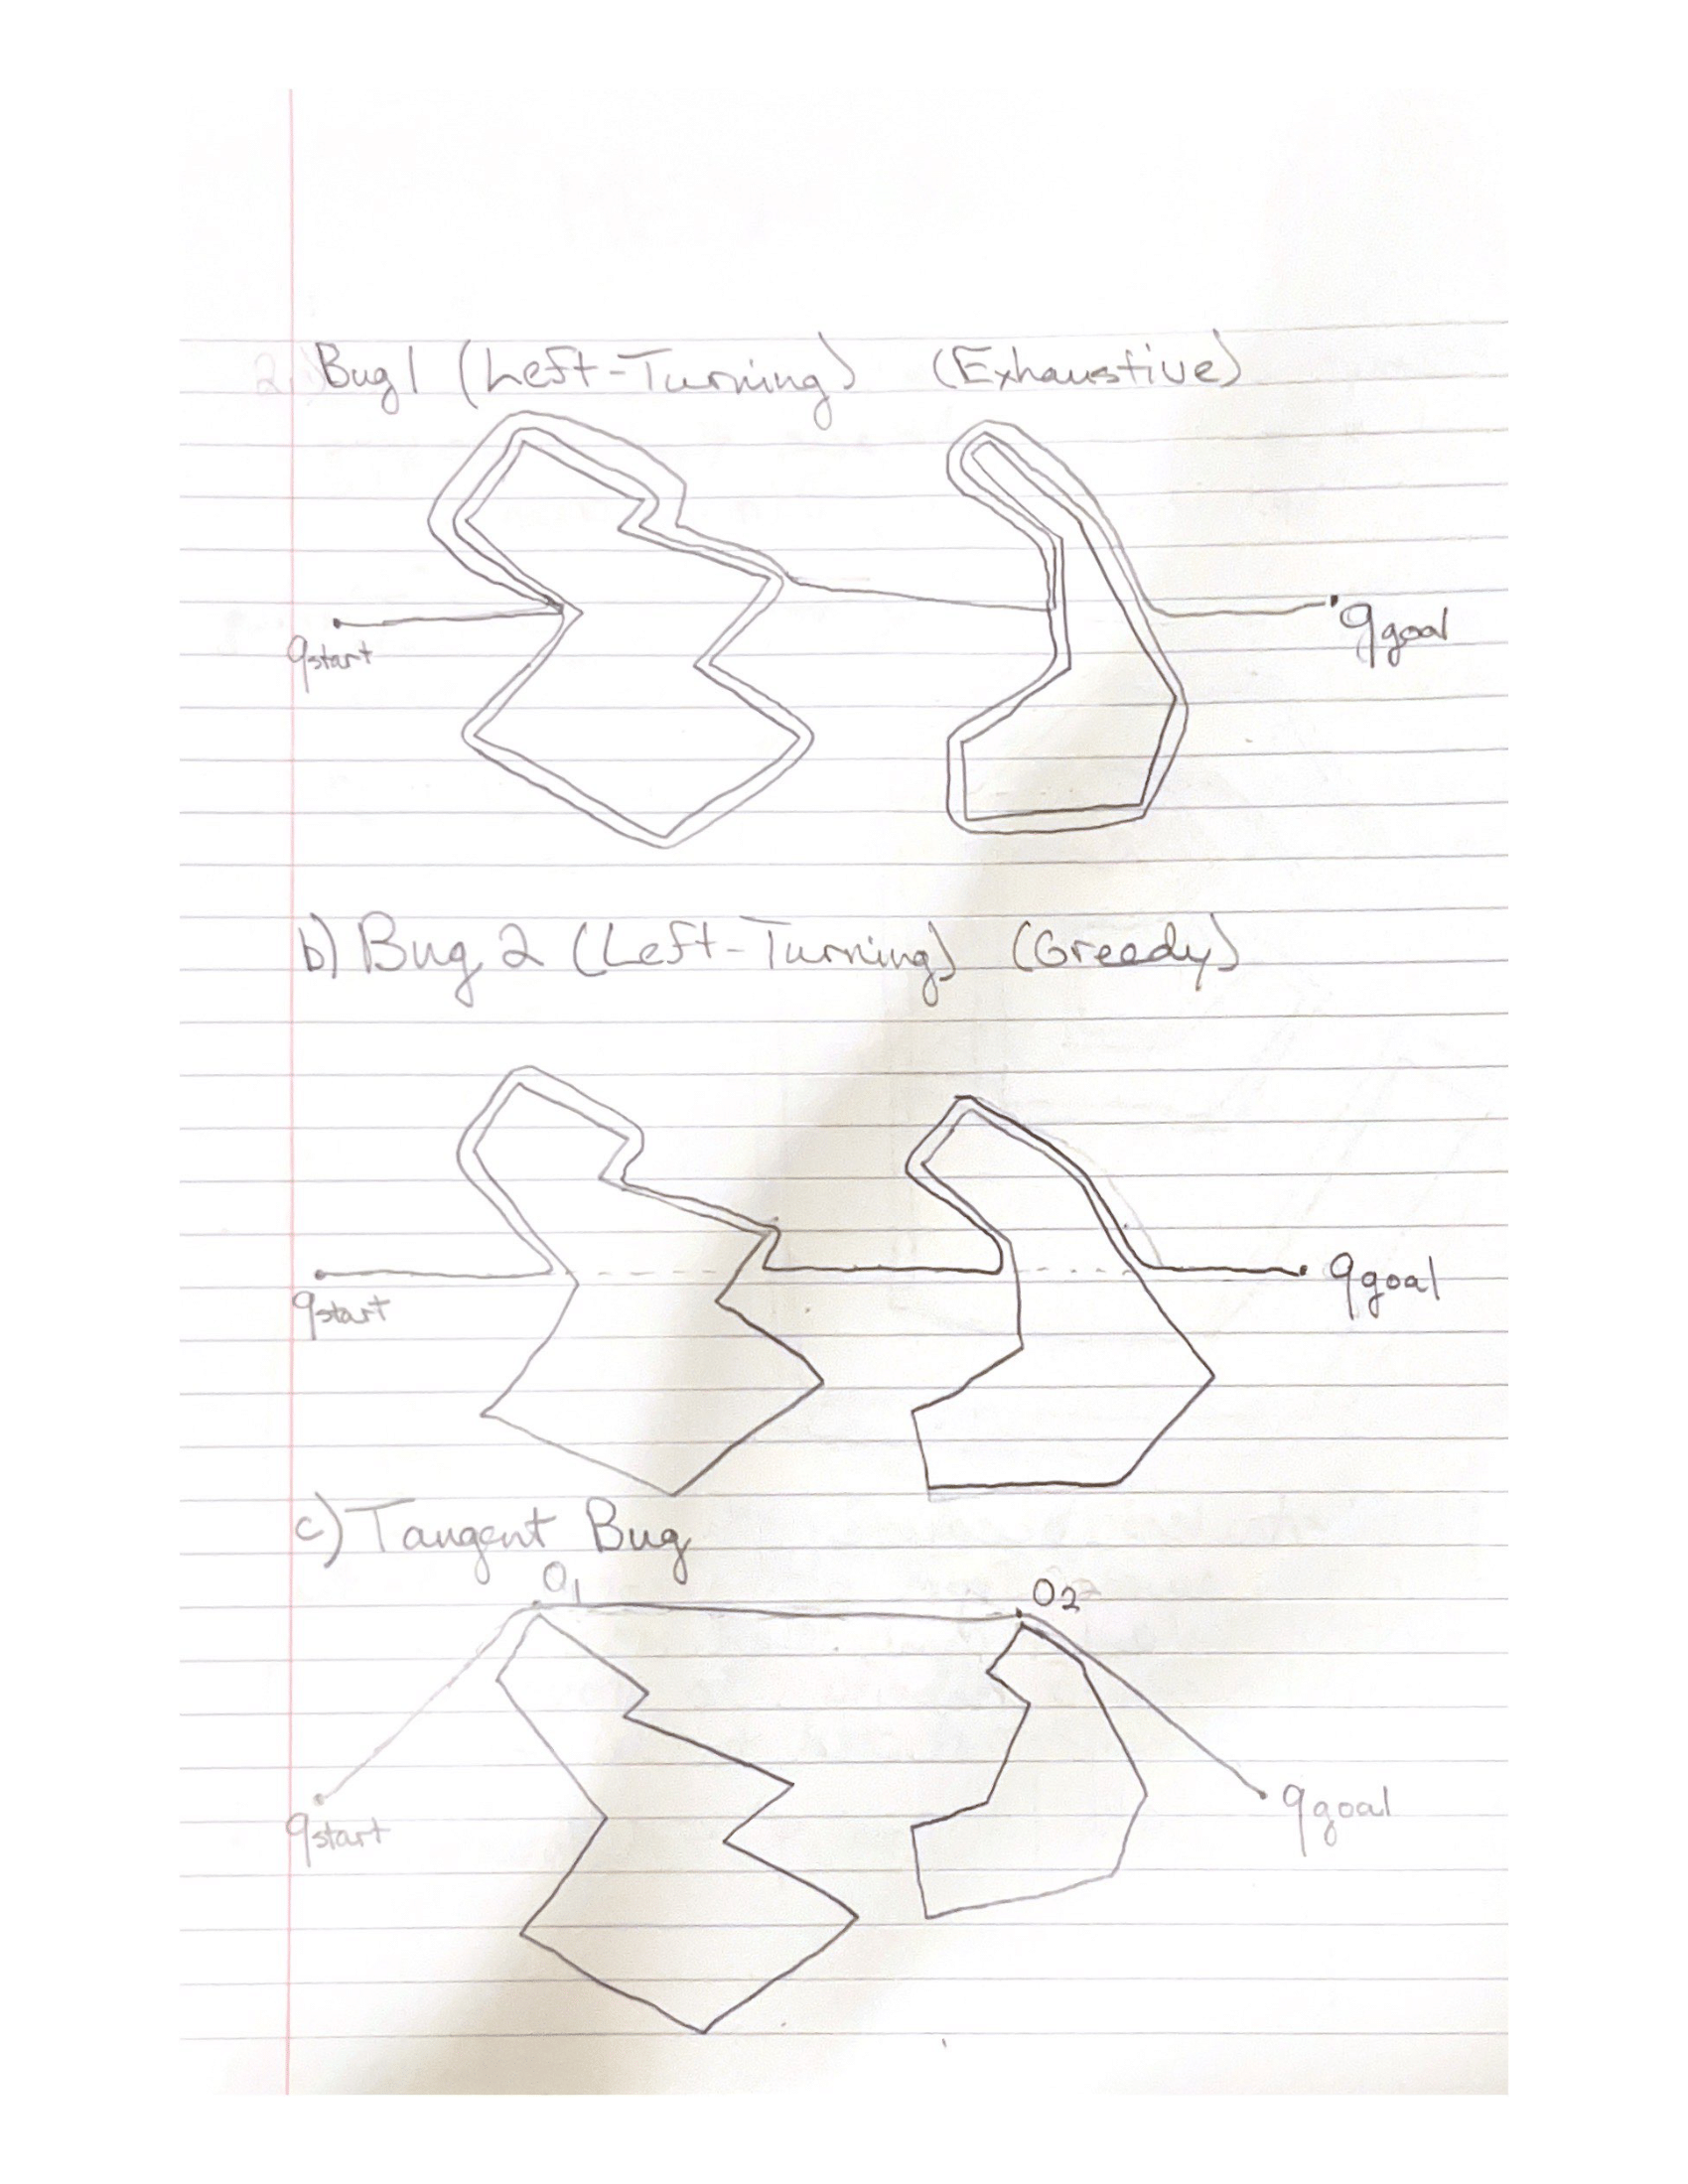
\includegraphics[width=11cm]{figures/problem2.png}
      \caption{Bug Trajectories}
      \label{fig:2}
   \end{figure}
    
  \end{enumerate}

  \newpage
  
  \item % Problem 3
  \begin{enumerate}
    Below in Figure \ref{fig:3}, an example for which the upper bound for the BUG 1 algorithm, $D +1.5P_1$ in this case, is achieved and the performance of BUG 2 is shown.   
  
   \begin{figure}[H]
      \centering
      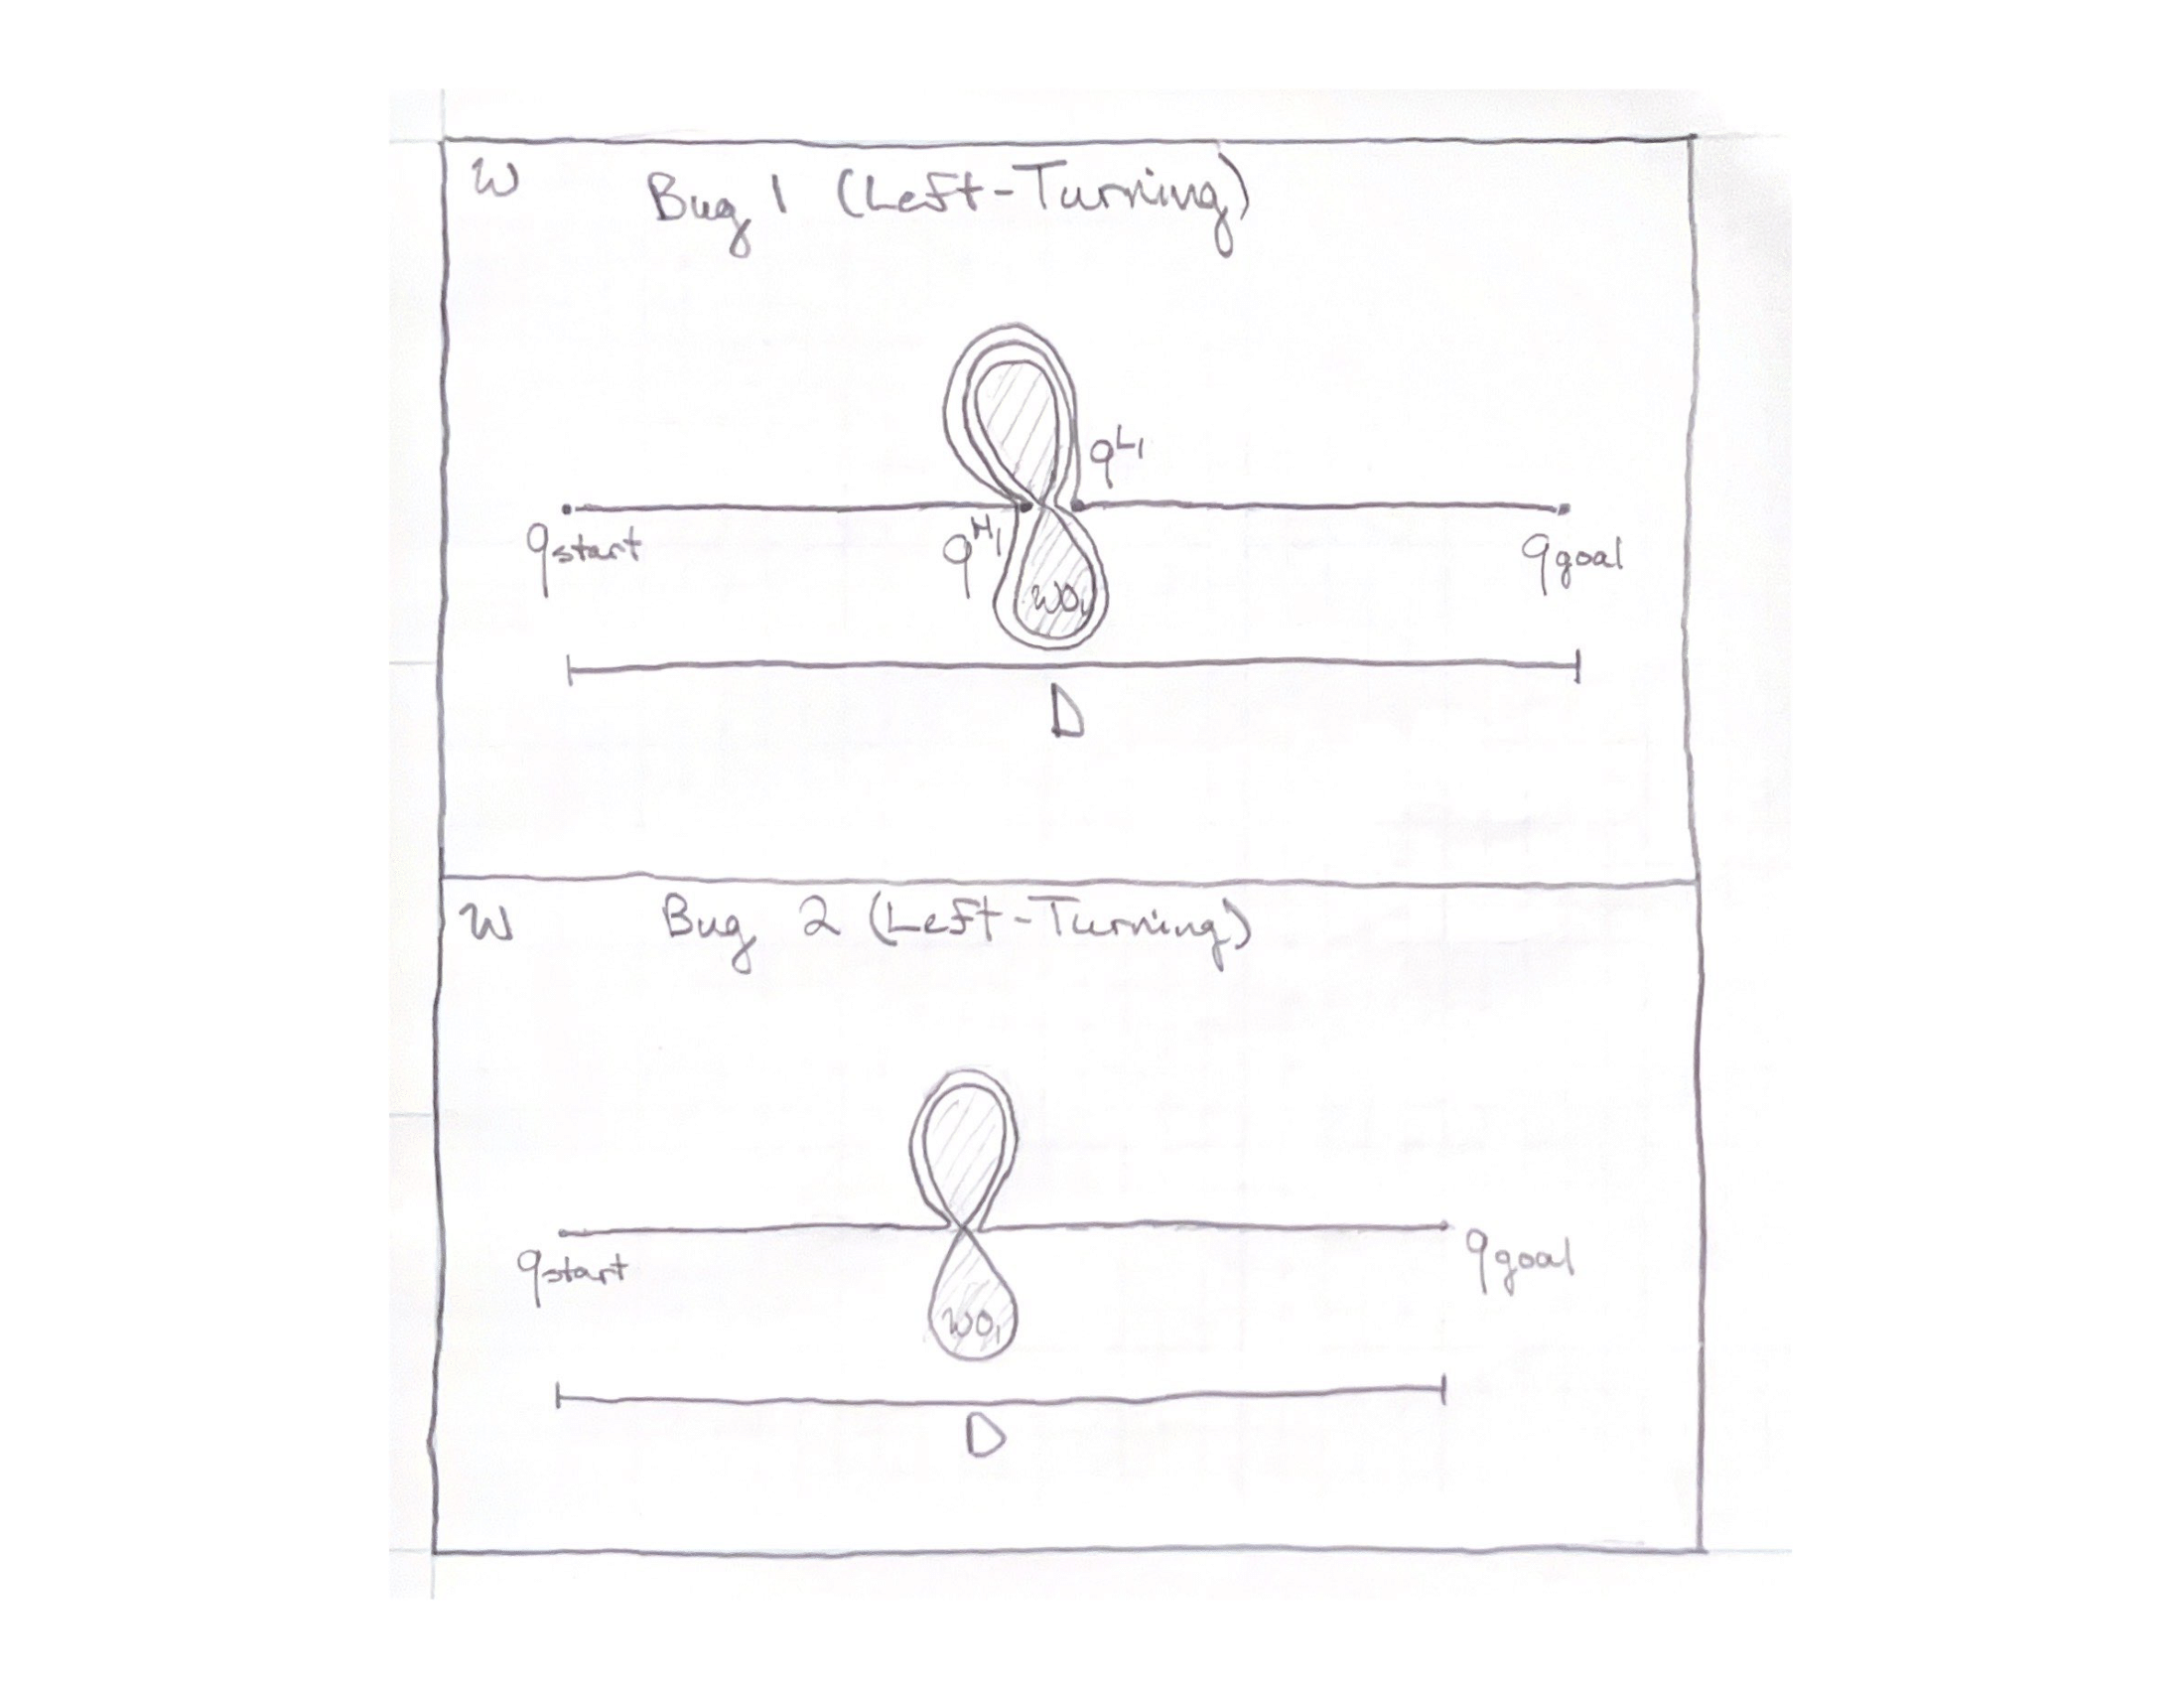
\includegraphics[width=12cm]{figures/problem3.png}
      \caption{BUG 1 Upper Bound}
      \label{fig:3}
   \end{figure}
    
    In this example, BUG 2 achieves a shorter path, since it only circles half of the obstacle $WO_1$ before returning to the m-line and reaching $q_{goal}$.
    
  \end{enumerate}

  \newpage

  \item %Problem 4
  \begin{enumerate}
    Below in Figure \ref{fig:4}, the paths from the Tangent Bug with the zero range detection and BUG 2 is given.
    
    \begin{figure}[H]
      \centering
      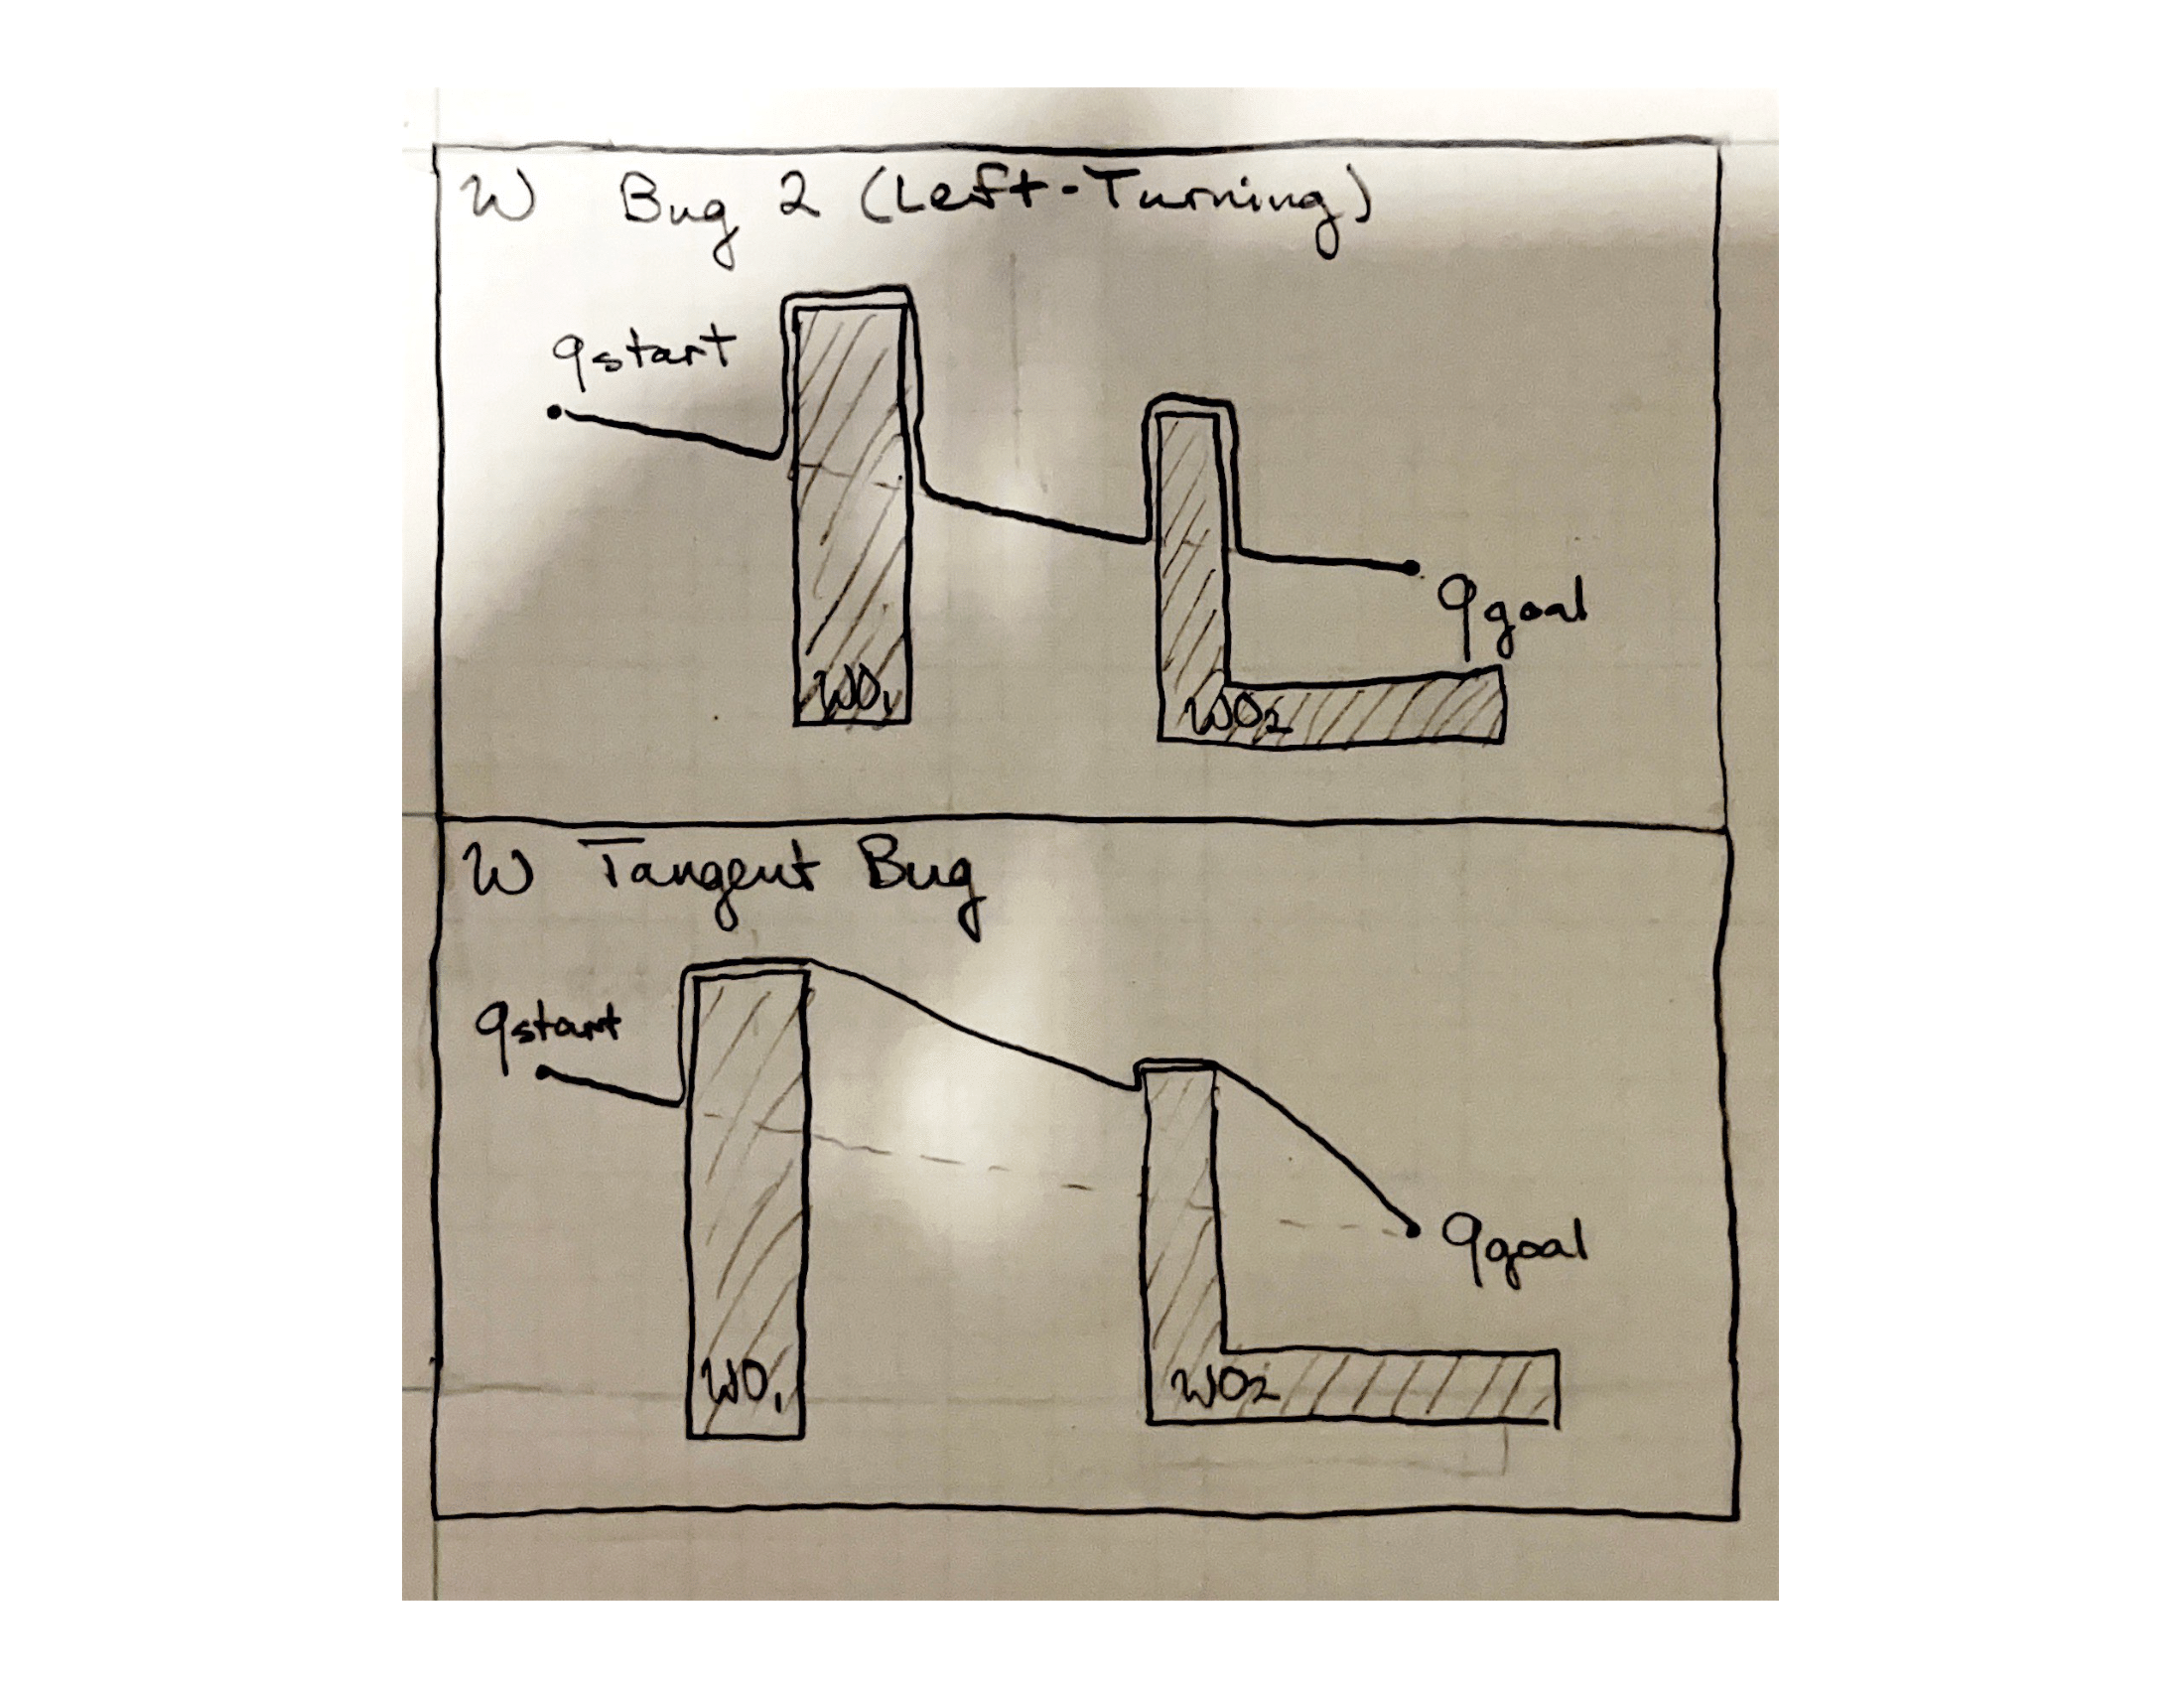
\includegraphics[width=12cm]{figures/problem4.png}
      \caption{Tangent Bug and BUG 2}
      \label{fig:4}
   \end{figure}

    One major difference between the Tangent Bug with zero range sensor and the BUG 2 algorithms is that the Tangent Bug algorithm does not return to the m-line, while the BUG 2 algorithms does. This can be clearly seen in the above example, as BUG 2 circles a larger portion of the obstacle perimeters to return to the m-line, while the tangent bug with zero sensor range immediately tries to go directly to the goal as soon as it no longer sees a blocking obstacle. As a result, the Tangent Bug circles a smaller portion of the obstacles in this example.
  \end{enumerate}
  
  \item %Problem 5
  \begin{enumerate}
    To prove the convergence of the Tangent Bug algorithm, we can use a proof by contradiction. Similar to the convergence proof for BUG 1, we can consider two cases.

    \begin{itemize}
      \item
      \item There exists a solution and the algorithm does not find it. \\ 
      \item There exists no solution, but the algorithm never terminates
    \end{itemize}
            For case 1 to be possible, it must be the case that the tangent bug cannot move towards the goal then cannot find a intermediate point $O_i$ that minimizes the heuristic distance to the goal, or the boundary-following cannot find a point on the obstacle such that $d_{reach} < d_{followed}$. We know that if some path to the goal exists and we are not boundary-following, then there is always an intermediate boundary point, $O_i$ such that the robot can minimize the heuristic distance to the goal, otherwise the robots would just move towards the goal freely. For the case where a path exists to the goal and we are boundary following, we can use the Jordan Curve Theorem to show that there exists a point on the obstacle so that $d_{reach} < d_{followed}$. For case 2 to be possible, it must be unknown that the robot has boundary followed the entire obstacle and still not found a point so that $d_{reach} < d_{followed}$ that allows it to move towards the goal again. But since this information is stored, this cannot be the case. Thus, we would arrive at a contradiction.
  \end{enumerate}
  
  \item %Problem 6
  \begin{enumerate}
      To prove that the shortest path is a polygonal path, we can use a proof by contradiction. Suppose we are a given shortest path $\tau$ that is not a polygonal path. By definition, for $\tau$ to globally be the shortest path between $p_{start}$ and $p_{goal}$, it is also locally the shortest path at some point $x_p$ in the free workspace that it intersects. At $x_p$, we can construct the ball centered at $x_p$, $B_r(x_p) = \{y \in \mathbb{R} | d(x_p, y) < r\}$, for some small radius, $r \in \mathbb{R}$. Now, if we have that the path formed by the intersection of $\tau$ with $B_r(x_p)$ is not a secant line through $B_r(x_p)$, then the path $\tau$ is not the shortest path through the ball $B_r(x_p)$, as a straight secant line would be shorter. Thus, we arrive at a contradiction, implying $\tau$ must be a polygonal path. $\square$ \break
      
      Next, we will prove that the inner vertices of the shortest path, $\tau$, are the vertices of $S$. We use a similar argument as before with a proof by contradiction. Suppose we are given the shortest path $\tau$ with inner vertex in the free workspace. We will denote the location of this vertex in the free workspace as $x_v$. We can construct the ball centered at $x_v$, $B(x_v) = \{y \in \mathbb{R} | d(x_v, y) < r\}$, with radius $r \in \mathbb{R}$ so that $B(x_v)$ is contained within the free workspace. Now, we could construct a shorter path within $B(x_v)$ by replacing the path with a vertex at $x_v$ with a secant line. Thus, we arrive at a contradiction, implying the shortest path must have vertices $x_v$ at vertices of $S$. $\square$ \break
  \end{enumerate}

\end{enumerate}

\end{document}
